\chapter{Ergebnisse} \label{chap:ergebnisse}

\section{Phylogenetische Strukturen und Klassifizierung} \label{sec:phylogenetische-strukturen}

Die phylogenetische Analyse der Flaviviridae-Familie, basierend auf den \gls{nsfive}-Sequenzen von 458 vollständigen Virengenomen, führte zu einer klaren Aufteilung in drei Hauptkladen. Die Maximum-Likelihood-Methode wurde zur Rekonstruktion des phylogenetischen Baumes verwendet, wobei das Substitutionsmodell \gls{gtrig} zum Einsatz kam. Die resultierende Topologie wurde durch hohe Bootstrap-Werte ($>$90\%) unterstützt und ermöglicht eine robuste Klassifizierung \autocite{mifsudMappingGlycoproteinStructure2024}.

Die erste Hauptklade umfasst klassische Vertreter der Gattung \textit{Flavivirus}, zu denen das Dengue-Virus, Zika-Virus und Gelbfieber-Virus gehören. Diese Gruppe zeigt eine bemerkenswerte Konservierung des NS5-Gens, was auf eine enge evolutionäre Verwandtschaft hindeutet. Die Glycoprotein-Strukturen, insbesondere das E-Glycoprotein, sind stark konserviert und spielen eine zentrale Rolle beim Eintritt in Wirtszellen \autocite{Rey1995}.

In der zweiten Hauptklade wurden die Gattungen \textit{Pegivirus} und \textit{Hepacivirus} zusammengefasst. Hier zeigt sich eine größere genetische Diversität, insbesondere in den Glycoprotein-Genen. Die strukturelle Variabilität der E1/E2-Glycoproteine deutet auf spezifische Mechanismen der Wirtsspezifität und des Viruseintritts hin \autocite{Vieyres2013}.

Die dritte Hauptklade vereint die Gattungen \textit{Pestivirus}, \textit{Jingmenvirus} und die sogenannten Large Genome Flaviviruses (LGFs). Diese Gruppe weist stark divergente Sequenzen und eine hohe strukturelle Vielfalt in den Glycoproteinen auf. Auffällig sind hier Anpassungen in transmembranen Domänen und möglichen Rezeptorbindungsstellen, die auf spezifische Wirt-Interaktionen hinweisen \autocite{Tautz2015}.

\section{Glycoprotein-Divergenz: Unterschiede zwischen Gattungen} \label{sec:glycoprotein-divergenz}

Die Vorhersage der Glycoprotein-Strukturen mithilfe von \gls{colabfold} und \gls{esmfold} zeigte sowohl konservierte als auch variable Merkmale zwischen den Hauptkladen.

Bei den \textit{Flaviviren} erwies sich das E-Glycoprotein als stark konserviert, insbesondere in der hydrophoben Fusion-Loop-Region und den transmembranen Domänen. Die typische Klasse-II-Faltungsarchitektur mit drei Domänen aus $\beta$-Faltblättern wurde bestätigt und unterstreicht die essenzielle Funktion dieser Region \autocite{Modis2004}.

Im Gegensatz dazu zeigten die Glycoproteine der \textit{Hepaciviren} und \textit{Pegiviren}, die aus E1/E2-Komplexen bestehen, signifikante strukturelle Unterschiede. Vor allem die Oberflächenexpositionen potenzieller Rezeptorbindungsstellen variieren stark und könnten die breite Wirtsspezifität und unterschiedliche Pathogenitätsprofile dieser Gattungen erklären \autocite{Lavie2017}.

\begin{figure}[H]
    \centering
    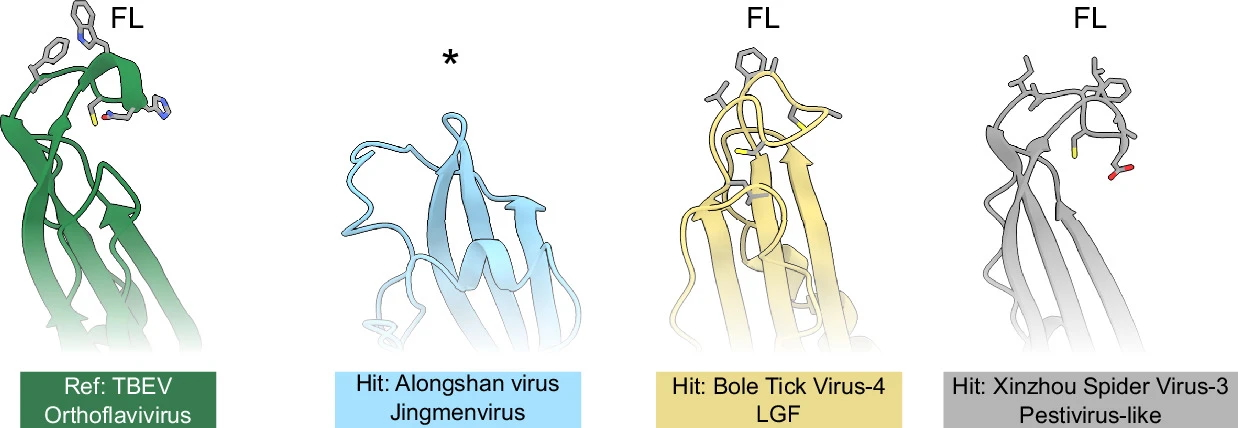
\includegraphics[width=\textwidth]{/workspaces/seminar-bioinformatik/images/figure6.jpeg}
    \caption{Strukturelle Unterschiede der Fusion-Loop-Regionen}
    \label{fig:figure6-orginal}
\end{figure}

Die größte strukturelle Diversität wurde in den Glycoproteinen der \textit{Pestiviren} und \textit{Jingmenviren} beobachtet. Unterschiede in der Anzahl und Position der transmembranen Domänen sowie Variationen in den extrazellulären Regionen deuten auf funktionelle Anpassungen hin, die spezifische Interaktionen mit Wirtsorganismen ermöglichen \autocite{Tautz2015}.

Trotz der beobachteten Variabilität wurden konservierte Motive wie die hydrophoben Fusion-Loops und transmembranen Segmente identifiziert, die für die grundlegende Funktion der Glycoproteine entscheidend sind und unter starkem Selektionsdruck stehen \autocite{Modis2004}.

\section{Spezifische Strukturmerkmale (Fusion-Loop und transmembrane Regionen)} \label{sec:spezifische-strukturmerkmale}

Die detaillierte Analyse der Fusion-Loop-Regionen und transmembranen Segmente der Glycoproteine lieferte wichtige Einblicke in deren funktionelle Rollen. Die Fusion-Loops bestehen aus konservierten hydrophoben Aminosäureresten, die essenziell für die Membranfusion sind. Bei den \textit{Flaviviren} zeigt die Fusion-Loop eine charakteristische Schleifenstruktur, die von Glycinresten flankiert wird und Flexibilität unter sauren pH-Bedingungen ermöglicht \autocite{Rey1995}. Im Gegensatz dazu deuten Unterschiede in Sequenz und Sekundärstruktur bei \textit{Hepaciviren} und \textit{Pegiviren} auf alternative Mechanismen der Membranfusion hin \autocite{Lavie2017}.

Die transmembranen Regionen variieren stark zwischen den Gattungen. Während \textit{Flaviviren} typischerweise nur eine einzelne transmembrane Domäne am C-Terminus des E-Glycoproteins besitzen, weisen \textit{Pestiviren} und \textit{Hepaciviren} mehrere transmembrane Segmente auf. Diese Variationen könnten die Organisation der Glycoproteine in der viralen Membran beeinflussen und somit die Virusassemblierung und -freisetzung modulieren \autocite{peninStructureFunctionMembrane2004}. Zusätzlich wurden Signalpeptide und Ankersequenzen identifiziert, die eine wichtige Rolle für die Lokalisierung und Stabilität der Proteine spielen \autocite{Ashkenazy2016}.